\documentclass[12pt]{article}

\usepackage{graphicx}
\usepackage{float}

\title{COSC 528: Project 4}
\author{Ian Lumsden}

\begin{document}
	\pagenumbering{gobble}
	\maketitle
	\newpage
	\pagenumbering{arabic}
	
	\section{Objective}
	The goal of this project was to classify emails as spam or not spam using the provided data. To do so, a neural network was implemented to attempt to classify the data. Then, the hyperparameters of the model were optimized using cross-validation. Finally, the dimensionality of the data was reduced using Principal Component Analysis (PCA), and the best neural net (as determined through cross-validation) was applied to this reduced data.
	
	\section{Preprocessing}
	No preprocessing was done to the data initially. This is because none of the data was invalid, and the data was already relatively normalized. Below is a description of the features in the data, as obtained from the spambase.names file.
	\begin{enumerate}
		\item \textbf{48 continuous real features} in the interval [0, 100] representing the percentage of times a specific word was in the email
		\item \textbf{6 continuous real features} in the interval [0, 100] representing the percentage of times a specific character was in the email
		\item \textbf{1 continuous real feature} representing the average length of uninterrupted sequences of capital letters
		\item \textbf{1 continuous real feature} representing the length of longest uninterrupted sequence of capital letters
		\item \textbf{1 continuous real feature} representing the total number of capital letters in the e-mail
		\item \textbf{1 nominal class attribute} that indicates whether the email was considered spam or not.
	\end{enumerate}
	
	\section{Neural Network}
	The only algorithm used for this project was the artificial neural network. My implementation of the neural net consisted of a single hidden layer (the size of the layer was a hyperparameter). Each hidden layer neuron used a leaky ReLU as the activation function. The output layer's activation function was allowed to be linear, softmax, or sigmoid and was decided by the user. Learning rate and training termination conditions were hyperparamters.
	
	\paragraph{}
	Sadly, this implementation worked \textbf{\textit{very}} poorly. After training and testing models using a very large number of permutations of hyperparameters, the best accuracy measure of any model was 0.6145494, which is extremely bad. Moreover, there were major issues for each type of output activation function. For softmax, the model would always classify data as the same class, regardless of whether it should be that class or not. For linear, the weights would get so large that overflow would occur, resulting in errors of NaN. For sigmoid, which was expected to be the best of the three, the model was not very accurate, but it performed with the most consistency. Additionally, only the softmax model ever produced better accuracy than sigmoid. However, since the outputs were more consistent for sigmoid, it is fair to say that it was the best model. Among sigmoid models, the following set of hyperparameters produced the most accurate model:
	\begin{table}[H]
		\centering
		\begin{tabular}{|c | c|}
			\hline
			Hyperparameters & Values\\ \hline
			Output Activation Function & Sigmoid \\
			Maximum Number of Iterations & 30 \\
			Error Threshold & 0.2 \\
			Error Change Threshold & 0.006 \\
			Learning Rate & 0.001 \\
			Number of Hidden Nodes & 40 \\ \hline
		\end{tabular}
		\caption{Best Hyperparamter Values}\label{hyper}
	\end{table}
	
	\section{Principal Component Analysis (PCA)}
	To try to improve the neural network, Principal Component Analysis was applied to the data.
	\paragraph{}
	To begin, the preprocessed data, $X$, was factored using singular value decomposition (SVD). This process converts the data into the following
	\begin{equation}
	X = U \Sigma V^T,
	\end{equation}
	where $U$ is an $m x m$ unitary matrix, $\Sigma$ is a diagonal $m x n$ matrix of eigenvalues, and $V$ is a $n x n$ unitary matrix of eigenvectors. The diagonal values of $\Sigma^2$ represent the variance that each principal component covers. By dividing by the sum of variances, the percentage of variance that each primary component covers was obtained. These percentages were plotted against the number of the principal component, as shown in Fig. \ref{Scree}.
	\begin{center}
		\begin{figure}[H]
			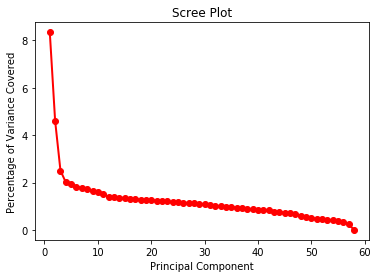
\includegraphics[width=0.75\linewidth]{scree.png}
			\caption{Scree Graph for SVD}
			\label{Scree}
		\end{figure}
	\end{center}
    From Fig. \ref{Scree}, the first three primary component clearly covered the most of the data's variance. However, the scree graph also suggests that the other components were also very important. The equations for PCA are as follows
    \begin{equation}
    W = XV^\prime = U^\prime S^\prime,
    \end{equation}
    where X is the initial dataset, the prime symbol indicates that a matrix has been reduced to its first $k$ columns, and W is the final reduced dataset.
    \paragraph{} 
    After reducing the data using this equation, the data was split into training and testing sets. A new model was trained using the hyperparamters determined previously through cross-validation. Then, the model was used to estimate the labels of the test set. However, the model incorrectly classified every test element. This was most likely caused by the various issues in the model (which will be discussed in the conclusion). However, part of the decrease in accuracy could be the result of the PCA. Since most of the elements have a non-negligible impact on the variance (see Fig. \ref{Scree}), reducing the dimensionality of the data could easily result in a non-negligible decrease in accuracy. 
    	
	\section{Conclusions}
	Overall, the neural network developed for this project failed to achieve its goal. The model could not accurately classify the email data for any combination of hyperparameters. The issue with the model likely stems from the implementation of backpropagation. The models with linear output activation functions suggest that the algorithm for evaluating the changes in weights was incorrect, as a correct implementation would not produce numeric overflow. Similarly, the fact that the softmax activation function caused the model to only output one class suggests that there could have been issues in the functions used as the derivatives of the activation functions. The softmax function is particularly suspect because several assumptions had to be made to simplify it as much as it was. In hindsight, these assumptions should \textbf{not} have been made. The largest likely issue with the backpropagation algorithm is that it was developed to reuse as much code as possible for each activation function. Due to the nature of the math behind backpropagation, there is a limited amount of code that can be reused for each activation function. The logic that I implemented to try to minimize the amount of code at least took away time that could have been spent on the algorithms themselves. At worst, this logic could have introduced their own sources of error. In the end, this model completely failed to classify the data and major improvements need to be made to the model for it to be useful.
	\pagebreak
	\section{Code}
	The following is a breakdown of the code files for this project:
	\begin{itemize}
		\item \textbf{driver.ipynb}: a Jupyter Notebook that is used as the "main" program
		\item \textbf{neuron.py}: the implementation of a single neuron
		\item \textbf{network.py}: the implementation of the neural network
		\item \textbf{PCA.py}: the implementation of PCA and its supporting and visualization functions
	\end{itemize}
\end{document}